\begin{prob}
	State TRUE or FALSE for the following statements:
	\begin{subprobset}
	    \begin{subprob}
    		If $(s, v_1, v_2, v_3, v_4)$ is a shortest path from $s$ to $v_4$ in a weighted graph, then $(s, v_1, v_2, v_3)$ is a shortest path from $s$ to $v_3$
    		\begin{responsebox}{1in}
    		    True. Assume for the sake of contradiction that there is a path P from s to $v_3$ whose weight is lesser than $(s, v_1, v_2, v_3)$. 
    		    Then we can find a path from s to $v_4$ by combining P with the edge ($v_3,v_4$) whose weight is lesser than $(s, v_1, v_2, v_3, v_4)$.
    		    This contradicts the fact that $(s, v_1, v_2, v_3, v_4)$ is a shortest path from $s$ to $v_4$.
    		\end{responsebox}
	    \end{subprob}
	    \begin{subprob}
    		Let P be a shortest path from some vertex s to some other vertex t in a directed graph. 
    		If the weight of each edge in the graph is increased by one, P will still be a shortest path from s to t.
    		\begin{responsebox}{1in}
    		    False. 
    		    \begin{center}
            	    	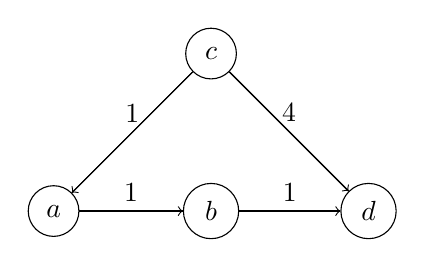
\begin{tikzpicture}
                		    \tikzset{
                   			vertex/.style={draw, circle, text width=8, align=center},
                    		arc/.style={->}
                		    }
    
               		    \draw node[vertex] (a) at (0,0) {$a$};
               		    \draw node[vertex] (b) at (2,0) {$b$};
      		            \draw node[vertex] (c) at (2,2) {$c$};
                		    \draw node[vertex] (d) at (4,0) {$d$};
        		            \foreach \x/\y in {%
        		        	    c/d, c/a,a/b,b/d%
       	         	    }{
                   		 	\draw (\x) edge[arc] (\y);
               		     }
    
                		    \draw[-] (c) -- node[above] {4} (d);
    			    \draw[-] (c) -- node[above] {1} (a);
    	 		    \draw[-] (a) -- node[above] {1} (b);
    			    \draw[-] (b) -- node[above] {1} (d);
            		\end{tikzpicture}
            	     \end{center}
                   	     Consider the graph given above. The shortest path from c to d is (c,a,b,d) which is of weight 3. 
    		     However, if the weight of each edge is increased by 1, the shortest path from c to d would be (c,d) of weight 5.
    		\end{responsebox}
	    \end{subprob}
	    \begin{subprob}
    		Suppose the update function is modified such the est[v] is updated when est[v] $\geq$ est[u] + weight(u,v) instead of strictly greater than.
    		The est values of all nodes at the end of the algorithm would still give the shortest distance from the source. 
    		\begin{responsebox}{1in}
    		    True. 
    		\end{responsebox}
	    \end{subprob}
	    \begin{subprob}
    		Suppose the update function is modified such the est[v] is updated when  est[v] $\geq$ est[u] + weight(u,v)  instead of strictly greater than.
    		We can still find the shortest path from the source to any node using the predecessors using the new algorithm. 
    		\begin{responsebox}{1in}
    		    False. 
    		    \begin{center}
            	    	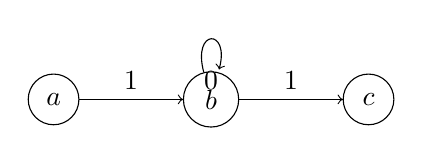
\begin{tikzpicture}
                		    \tikzset{
                   			vertex/.style={draw, circle, text width=8, align=center},
                    		arc/.style={->}
                		    }
    
               		    \draw node[vertex] (a) at (0,0) {$a$};
               		    \draw node[vertex] (b) at (2,0) {$b$};
      		            \draw node[vertex] (c) at (4,0) {$c$};
                		    
        		            \foreach \x/\y in {%
        		        	    a/b,b/c%
       	         	    }{
                   		 	\draw (\x) edge[arc] (\y);
               		     }
    				\draw (b) edge[loop above] (b);
    			    \draw[-] (b) -- node[above] {0} (b);
    	 		    \draw[-] (a) -- node[above] {1} (b);
    			    \draw[-] (b) -- node[above] {1} (c);
            		\end{tikzpicture}
            	     \end{center}
    		     Consider the graph given above. Let a be the source in the execution of Bellman Ford algorithm.
    		     Updating the edge will result in est[b] = 1 and predecessor[b] = a.
    		     However, updating the edge (b,b) will result in predecessor[b] = b according to the new update algorithm.
    		     Therefore, it would not be possible to find the shortest path from a to b using the predecessors.
    		\end{responsebox}
	    \end{subprob}
	\end{subprobset}
\end{prob}
